\documentclass{article}
\pdfpagewidth=8.5in
\pdfpageheight=11in

\usepackage{../WMHreport}
% Use the postscript times font!
\usepackage{times}
\usepackage{soul}
\usepackage{url}
\usepackage{xcolor}
\usepackage{polski}
\usepackage[polish]{babel}
\usepackage[utf8]{inputenc}
\usepackage[T1]{fontenc}
\usepackage[utf8]{luainputenc}
\usepackage[hidelinks]{hyperref}
\usepackage[utf8]{inputenc}
\usepackage{caption}
\usepackage{indentfirst}
\usepackage{graphicx}
\usepackage{amsmath}
\usepackage{siunitx}
\usepackage{booktabs}
\usepackage{subfig}

\urlstyle{same}
	
\title{Współczesne metody heurysytczne\\ Sprawozdanie zerowe z projektu}

\author{
Julia Kłos, Jakub Sikora
\affiliations
numery albumów: 283607, 283418 \\
\emails
julia.klos.stud@pw.edu.pl, jakub.sikora2.stud@pw.edu.pl
}

\newcommand{\todo}[1]{\textcolor{red}{\textbf{TO DO:} #1}}

\begin{document}
\maketitle

\section{Temat projektu}
\label{sec:temat}
Tematem projektu jest zastosowanie maszyny wektorów nośnych w~zadaniu aproksymacyjnym. W~ramach zadania projektowego, należy zaprojektować maszynę wektorów nośnych do aproksymacji ciągłej funkcji dwuwymiarowej. Maszyna powinna nauczyć się określonej liczby punktów, a~następnie prawidłowo (z~akceptowalnym błędem) aproksymować punkty z~drugiego zbioru (testowego). Projekt powinien obejmować wypróbowanie różnych struktur maszyny (różne funkcje jądrowe, liczba funkcji jądrowych i~dobranie ich parametrów) oraz określenie struktury optymalnej dla problemu. Należy zbadać również proces uczenia maszyny.

\section{Propozycja rozwiązania}
\label{sec:rozwiazanie}
Do aproksymacji wygenerowanych danych wykorzystany zostanie algorytm SVR zaimplementowany w ramach bilioteki \textit{scikit-learn} języka Python. Dla różnych poziomów zaszumienia danych zbadany zostanie błąd przybliżenia funkcji przy użyciu różnych funkcji jądrowych:
\begin{itemize}
    \item liniowej,
    \item wielomianowej,
    \item radialnej (\textit{rbf}),
    \item sigmoidalnej.
\end{itemize}

Dla każdej funkcji jądrowej poszukiwany będzie parametr regularyzacji $C$ oraz parametr marginesu błędu $\epsilon$. Oprócz tego, dla każdej funkcji jądrowej dobierane będą parametry specyficzne dla danej funkcji parametry; parametr $\gamma$ (wielomianowa, radialna, sigmoidalna), stopień wielomianu (tylko wielomianowa) i~wyraz wolny (wielomianowa i~sigmoidalna).\\

Jakość aproksymacji zostanie oceniona przy użyciu K-krotnej walidacji krzyżowej. Oznacza to, że dane zostaną podzielone na K rozłącznych pozbiorów. Każdy z nich zostanie wykorzystany jako zbiór testowy, a pozostałe podzbiory razem-- jako zbiór uczący. Wyniki z K analiz zostaną następnie uśrednione. Błędy zdefiniowane zostaną poprzez:
\begin{itemize}
    \item błąd średniokwadratowy ($MSE$),
    \item średni błąd względny ($MAE$),
    \item współczynnik determinacji ($R^2$).
\end{itemize}


\section{Dane}
\label{sec:dane}
Projektowana maszyna wektorów nośnych będzie aproksymowała następującą funkcję:

\begin{equation}
    \label{eqn:fun}
    f(x,y) = \log_{10}{|x|} \cos{y} + 0,55(x+y)
\end{equation}
\smallskip

Wykres funkcji \ref{eqn:fun} został przedstawiony na rysunku \ref{fig:fun}. W projekcie zbadany zostanie wpływ nałożenia białego, gaussowskiego szumu addytywnego o różnej mocy $\sigma$ na oryginalną funkcję.

\begin{figure}
    \centering
    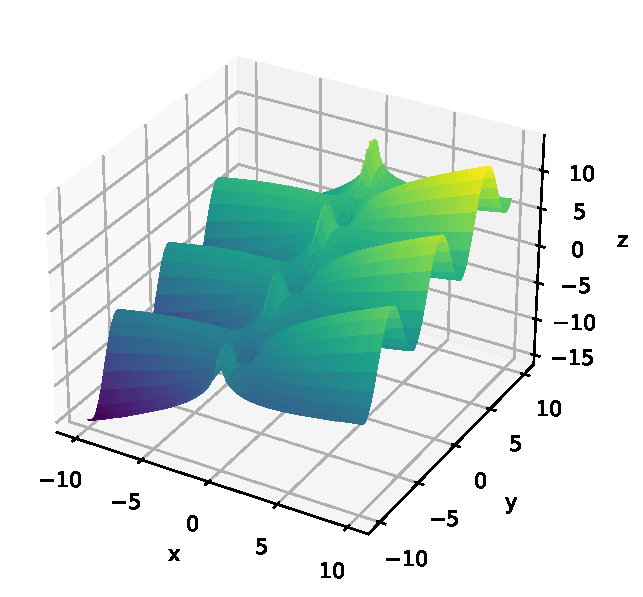
\includegraphics{./figures/fun.pdf}
    \caption{Wykres aproksymowanej funkcji dwuwymiarowej}
    \label{fig:fun}
\end{figure}

\end{document}